\documentclass[a4paper,12pt,titlepage]{article}

%Εισαγωγή γλωσσικής υποστήριξης
%ελληνικό hyphenation

\usepackage{fontspec}
\usepackage{xunicode}
\usepackage{xltxtra}
\usepackage{xgreek}
\usepackage[colorlinks]{hyperref}
\usepackage{enumerate}
\usepackage{amsmath}
%\usepackage{tikz}
%η γραμματοσειρά
%\setmainfont[Mapping=tex-text]{Times New Roman} %απλοποιημένο σε σχέση με το άρθρο
\setmainfont[Mapping=tex-text]{Linux Libertine} 
%page orientation
\usepackage{a4wide}
\voffset = -0.5in
\textheight = 664pt

%Άλλα χρήσιμα πακέτα
\usepackage{graphicx} 	%εισαγωγή εικόνων jpg/png κλπ
\usepackage{listings}
\lstset{commentstyle=\textit,
captionpos=b,
breakatwhitespace=true,
showstringspaces=false,
breaklines=true,
keywordstyle=\color{black}\bfseries,
float=htb,
frame=single}

%απενεργοποίηση του indent στις νέες παραγράφους
\parindent=0in

%macro που δίνει το μέγιστο επιτρεπτό μέγεθος σε μια εικόνα χωρίς να παραβιάζει τα όρια του LaTeX
\makeatletter
\def\maxwidth{
\ifdim\Gin@nat@width>\linewidth
\linewidth
\else
\Gin@nat@width
\fi
}

\makeatother

\title{1η Άσκηση\\kn}
\author{AxiP}
\date{\today}

\begin{document}

\pagestyle{headings}    %αρίθμηση στο πάνω μέρος της σελίδας

%\maketitle
\begin{titlepage}
\begin{center}

\includegraphics[width=50mm]{pyrforos.pdf}\\[0.5cm]
\textbf{\LARGE ΕΘΝΙΚΟ ΜΕΤΣΟΒΙΟ ΠΟΛΥΤΕΧΝΕΙΟ}\\
\textrm{\Large Σχολή Εφαρμοσμένων Μαθηματικών και Φυσικών Επιστημών}\\[2.0cm]
\Huge{Τεχνολογία των laser\\}
\Large{\textit{6o εξάμηνο, ΣΕΜΦΕ}}\\[2.0cm]
\Large{\textit{\textbf{Κατασκευή τροφοδοτικού διοδικού laser}}}\\[5.0cm]
\normalsize

\begin{minipage}{0.49\textwidth}
\begin{flushleft}
\textbf{Αχιλλέας Πιπινέλλης}, 09103163
\end{flushleft}
\end{minipage}
\begin{minipage}{0.49\textwidth}
\begin{flushright}
\textbf{\\
\textit{Η/Μ Παράδοσης:} 2 Ιουνίου 2012}
\end{flushright}
\end{minipage}

%\maketitle

\vfill
%bottom of the page
{Αθήνα, 2012}

\end{center}
\end{titlepage}

\section{Σκοπός του πειράματος}

Στην παρούσα άσκηση θα εξετάσουμε πως δουλεύει ένα διοδικό laser και θα μελετήσουμε τη σταθεροποίηση του ρεύματος, εργαζόμενοι πάνω σε ένα breadborad του οποίου τα εξαρτήματα θα απαριθμήσουμε παρακάτω.

\section{Θεωρία}

\subsection*{Διοδικό Laser}

\begin{figure}[!h]
\centering
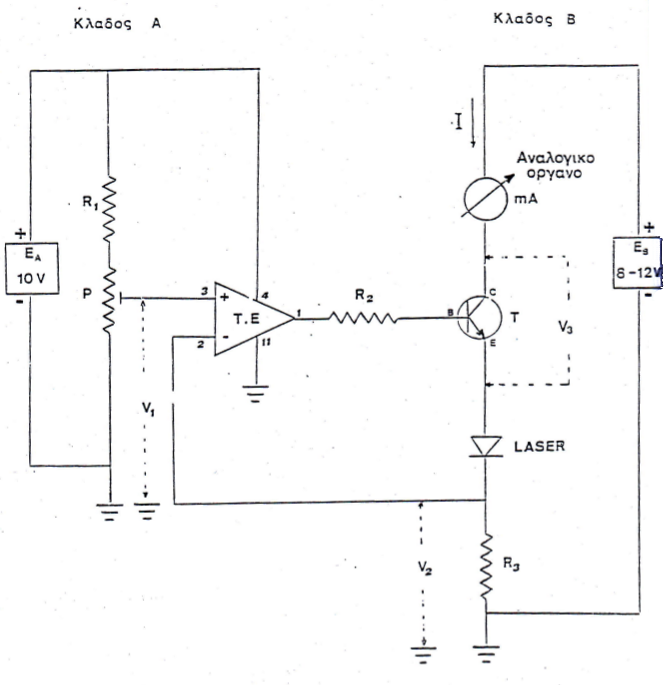
\includegraphics[width=\maxwidth]{diataksi.png}\\[0.3cm]
\end{figure}

\newpage

\section{Μέθοδος}

\subsection{Πειραματική Διάταξη}

Η άσκηση θα εκτελεστεί σε  πλακέτα γενικών κατασκευών (breadborad). H διάταξη του πειράματος περιλαμβάνει τα εξής εξαρτήματα:

\begin{itemize}
  \item Δύο τροφοδοτικά χαμηλής τάσεως($E_{A}=10V$, $E_{B}=15V$) τα οποία τροφοδοτούν τους κλάδους Α και Β αντίστοιχα (βλ. Σχήμα 1).
  \item Αναλογικό όργανο για τη μέτρηση του ρεύματος $Ι$ του laser.
  \item Ψηφιακό όργανο για τη μέτρηση των τάσεων $V_{1}$, $V_{2}$, $V_{3}$.
  \item Μία δίοδο laser.
  \item Ένα ολοκληρωμένο κύκλωμα.
  \item	Έναν ημιαγωγό.
  \item Τρεις αντιστάσεις $R_{1}$, $R_{2}$, $R_{3}$.
  \item	Ένα ποτενσιόμετρο.
  \item	Μία πλακέτα (breadboard).
\end{itemize}

\newpage

\section{Εκτέλεση}

Ρυθμίσαμε την τάση $E_{B}=10V$ και μεταβάλαμε την τάση $V_{1}$ με το ποτενσιόμετρο από $0V-4.5V$ με βήμα $0.5V$. Τα αποτελέσματα παρουσιάζονται στον πίνακα 1.

\begin{table}[h!]
\begin{center}
    \begin{tabular}{ | c | c |}
    \hline
     $V_{1} (Volt)$ & $V_{2} (Volt)$\\ \hline
     0	  &   0\\ \hline
     0.49 & 5.0\\ \hline
     0.99 & 5.0\\ \hline
     1.51 & 5.0\\ \hline
     2.01 & 4.8\\ \hline
     2.52 & 4.6\\ \hline
     3.01 & 4.2\\ \hline
     3.49 & 4.0\\ \hline
     4.02 & 3.8\\ \hline
     4.50 & 3.7\\ \hline
    \end{tabular}
\end{center}
\caption{Τάση $V_{1}$, $V_{2}$ με $E_{B}=10V$ }
\end{table}

Παρατηρούμε πως δεν υπάρχει διαφορά τάσης, άρα ο τελεστικός ενισχυτής διατηρεί τις δύο τάσεις ίσες.

\newpage

Στη συνέχεια ρυθμίσαμε το ρεύμα μέσω του ποτενσιόμετρου να είναι $35mA$ και μεταβάλλοντας την τάση της πηγής $E_{B}$ από $8V-12V$ με βήμα $0.5V$ μετρήσαμε πως μεταβάλλεται το ρεύμα συναρτήσει της τάσης. Το ίδιο κάναμε και για $I=45mA$. Όπως παρατηρεί κανείς, το ρεύμα και στις δύο περιπτώσεις παραμένει το ίδιο. Τα αποτελέσματα παρουσιάζονται στον Πίνακα 2 και το Σχήμα 1.

\begin{table}[h!]
\begin{center}
    \begin{tabular}{ | c | c | c |}
    \hline
     $E_{B}(Volt)$ & $I_{35} (mA)$ & $I_{45} (mA)$\\ \hline
     8.0  & 35	& 45 \\ \hline
     8.5  & 35	& 45 \\ \hline
     9.0  & 35	& 45 \\ \hline
     9.5  & 35	& 45 \\ \hline
     10.0 & 35	& 45 \\ \hline
     10.5 & 35	& 45 \\ \hline
     11.0 & 35	& 45 \\ \hline
     11.5 & 35	& 45 \\ \hline
     12.0 & 35	& 45 \\ \hline
    \end{tabular}
\end{center}
\caption{Μεταβολή του ρεύματος $I$ συναρτήσει της τάσης $E_{B}$}
\end{table}

\begin{figure}[!h]
\centering
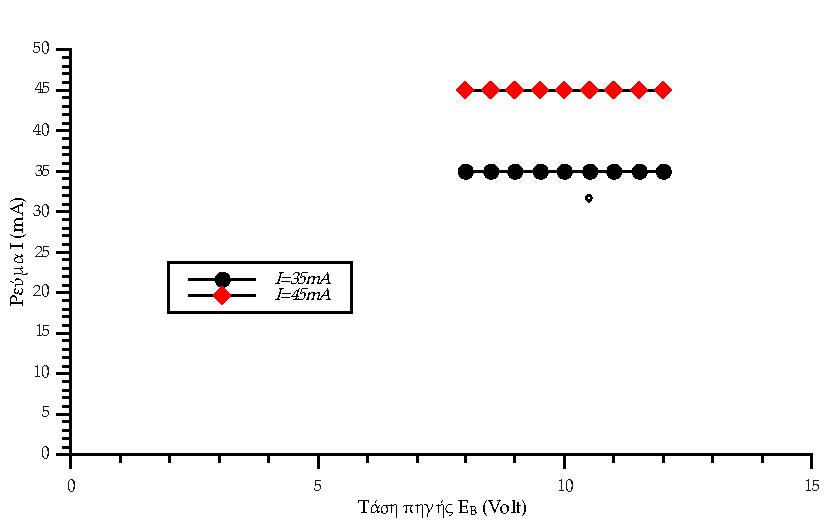
\includegraphics[width=\maxwidth]{graph1.pdf}\\[0.3cm]
\caption{Μεταβολή του ρεύματος $I$ συναρτήσει της τάσης $E_{B}$}
\end{figure}

\newpage

Ρυθμίζοντας το ρεύμα σταθερό στα $40 mA$, μεταβάλαμε την τάση $E_{B}$ απο $8V-12V$ με βήμα $0.5$ και πήραμε μετρήσεις των τάσεων $V_{2}$ και $V_{3}$. Τα αποτελέσματα φαίνονται στον πίνακα 3.

\begin{table}[h!]
\begin{center}
    \begin{tabular}{ | c | c | c |}
    \hline
     $E_{B}(Volt)$ & $V_{2} (Volt)$ & $V_{3} (Volt)$\\ \hline
     8.0  	& 2.65	& 3.20 \\ \hline
     8.5  	& 3.04	& 3.18 \\ \hline
     9.0  	& 3.78	& 3.15 \\ \hline
     9.5  	& 4.30	& 3.15 \\ \hline
     10.0 	& 4.90	& 3.14 \\ \hline
     10.5 	& 5.71	& 3.14 \\ \hline
     11.0 	& 6.25	& 3.14 \\ \hline
     11.5 	& 6.77	& 3.14 \\ \hline
     12.0 	& 7.32	& 3.13 \\ \hline
    \end{tabular}
\end{center}
\caption{Μεταβολή των τάσεων $V_{2}$ και $V_{3}$ συναρτήσει της τάσης $E_{B}$ για $I=40mA$}
\end{table}

Παρατηρούμε πως η τάση $V_{2}$

\end{document}